\documentclass[aspectratio=169]{beamer}

\usepackage[utf8]{inputenc}
\usepackage[T1]{fontenc}
\usepackage{tikz}
\usepackage{booktabs}
\usepackage{xcolor}
\usepackage{tcolorbox}
\tcbuselibrary{skins}
\usepackage{graphicx}
\usepackage{hyperref}
\usetikzlibrary{positioning, arrows.meta, calc, decorations.pathreplacing}

%% -- same theme and colours as "Deep Learning for Maritime Vision Applications" --
\usetheme[nofirafonts]{pureminimalistic}
\renewcommand{\logoheader}{}
\renewcommand{\logotitle}{}
\newcommand{\institutepath}{}
\renewcommand{\logofooter}{}

\definecolor{marineblue}{RGB}{51,65,133}
\definecolor{marinelight}{RGB}{101,115,183}
\definecolor{exercisebg}{RGB}{232,236,250}
\definecolor{accentorange}{RGB}{220,100,30}
\definecolor{accentgreen}{RGB}{40,150,90}
\definecolor{accentred}{RGB}{180,30,40}
\definecolor{lightgray}{RGB}{245,245,245}
\definecolor{darkgray}{RGB}{80,80,80}

\newtcolorbox{infobox}[1]{%
  enhanced, colback=lightgray, colframe=marinelight,
  fonttitle=\bfseries, title={#1}, arc=3pt,
  left=4pt, right=4pt, top=3pt, bottom=3pt}

%% open question box for the students (orange = "hands-on" colour of the course)
\newtcolorbox{ideabox}[1]{%
  enhanced, colback=accentorange!8, colframe=accentorange,
  coltitle=white, colbacktitle=accentorange,
  fonttitle=\bfseries, title={#1}, arc=3pt,
  left=4pt, right=4pt, top=3pt, bottom=3pt}

\title{Can a computer identify deep-sea animals?}
\subtitle{FathomNet project}
\author{Torben Globisch}

\begin{document}
%% =====================================================================
%% Two motivation slides: "Why CNNs?" and "The FathomNet 2025 Challenge".
%% Drop into any pureminimalistic deck with %% =====================================================================
%% Two motivation slides: "Why CNNs?" and "The FathomNet 2025 Challenge".
%% Drop into any pureminimalistic deck with %% =====================================================================
%% Two motivation slides: "Why CNNs?" and "The FathomNet 2025 Challenge".
%% Drop into any pureminimalistic deck with \input{fathomnet_frames}
%% (needs the colours and the infobox/ideabox from fathomnet_motivation.tex).
%% =====================================================================

%% ---- Slide 1: Why CNNs? ----
\begin{frame}{Why CNNs? \,--\, Teaching a computer to look like a biologist}
\begin{columns}[T]
\begin{column}{0.56\linewidth}
  \centering
  \begin{tikzpicture}[
      every node/.style={font=\scriptsize},
      layer/.style={draw=marineblue, fill=marineblue!15, minimum width=0.42cm},
      arr/.style={-{Stealth[scale=0.8]}, thick, marineblue}]
    \node[inner sep=0, draw=marineblue, line width=0.8pt] (img) at (0,0)
      {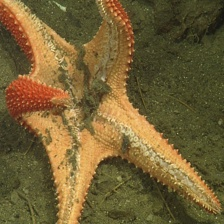
\includegraphics[width=1.7cm]{img/animal1}};
    \node[layer, minimum height=1.45cm] (l1) at (1.55,0) {};
    \node[layer, minimum height=1.05cm, fill=marineblue!30] (l2) at (2.55,0) {};
    \node[layer, minimum height=0.65cm, fill=marineblue!50] (l3) at (3.55,0) {};
    \node[draw=accentorange, fill=accentorange!12, rounded corners=3pt, align=center,
          font=\scriptsize\bfseries, text=accentorange] (out) at (5.0,0) {sea star\\[-1pt]\textit{Hippasteria}};
    \draw[arr] (img) -- (l1); \draw[arr] (l1) -- (l2);
    \draw[arr] (l2) -- (l3);  \draw[arr] (l3) -- (out);
    \foreach \x/\t in {0/ROV image, 1.55/edges, 2.55/{spines,\\[-2pt]textures}, 3.55/{arms,\\[-2pt]body plan}}
      \node[anchor=north, align=center, darkgray, text width=1.1cm] at (\x,-0.9) {\t};
  \end{tikzpicture}\\[6pt]
  \raggedright\small
  \begin{itemize}
    \item \textbf{Too much footage, too few experts.} Underwater robots film for
          hours on every dive -- labelling it by hand is the bottleneck.
    \item \textbf{A CNN learns its own characters} -- edges $\to$ textures $\to$ body
          parts -- from labelled examples, much like a student learning an
          identification key.
    \item \textbf{It does not replace you:} the CNN pre-sorts, the biologist checks.
  \end{itemize}
\end{column}
\begin{column}{0.40\linewidth}
  \begin{infobox}{It already works in this project}
    \small
    A ready-made CNN + a simple classifier, 79 deep-sea taxa:\\[4pt]
    \begin{tabular}{@{}lr@{}}
      guessing the commonest label & \textbf{1\,\%}\\
      raw pixels                   & \textbf{46\,\%}\\
      CNN features                 & \textbf{\textcolor{accentgreen}{65\,\%}}\\
    \end{tabular}\\[4pt]
    {\scriptsize\color{darkgray} our reference run, random test split}
  \end{infobox}
  \vspace{4pt}
  \begin{ideabox}{Your turn}
    \small Which characters do \emph{you} use to tell two species apart --
    and could a camera even see them?
  \end{ideabox}
\end{column}
\end{columns}
\end{frame}

%% ---- Slide 2: The FathomNet 2025 challenge ----
\begin{frame}{The FathomNet 2025 Challenge}
\begin{columns}[T]
\begin{column}{0.47\linewidth}
  \centering
  \setlength{\tabcolsep}{1pt}\renewcommand{\arraystretch}{0}
  \begin{tabular}{cccc}
    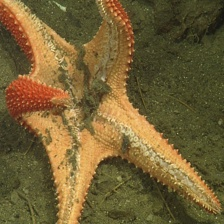
\includegraphics[width=1.55cm,height=1.55cm]{img/animal1} &
    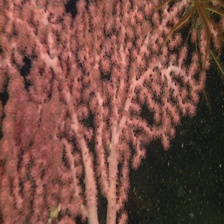
\includegraphics[width=1.55cm,height=1.55cm]{img/animal2} &
    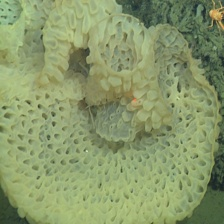
\includegraphics[width=1.55cm,height=1.55cm]{img/animal3} &
    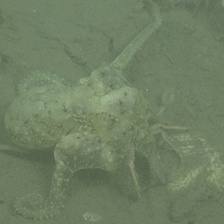
\includegraphics[width=1.55cm,height=1.55cm]{img/animal4} \\[1pt]
    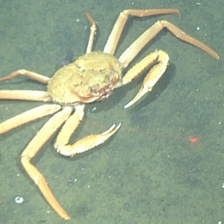
\includegraphics[width=1.55cm,height=1.55cm]{img/animal5} &
    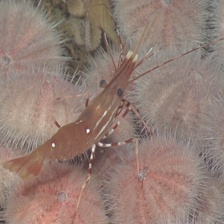
\includegraphics[width=1.55cm,height=1.55cm]{img/animal6} &
    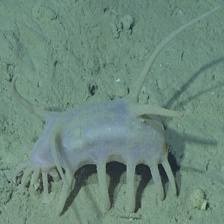
\includegraphics[width=1.55cm,height=1.55cm]{img/animal7} &
    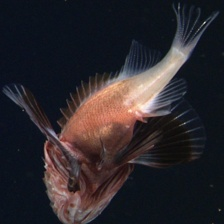
\includegraphics[width=1.55cm,height=1.55cm]{img/animal8} \\
  \end{tabular}\\[5pt]
  {\tiny\color{darkgray} sea star · bubblegum coral · glass sponge · octopus ·
   crab · prawn · sea pig · rockfish \quad (images: FathomNet / MBARI)}\\[6pt]
  \raggedright\small
  \textbf{\color{marineblue}23{,}664} expert-labelled animals \;·\;
  \textbf{\color{marineblue}79} taxa \;·\; \textbf{\color{marineblue}7} phyla \;·\;
  \textbf{\color{marineblue}1{,}465} ROV dives
\end{column}
\begin{column}{0.49\linewidth}
  \small
  \textbf{The task:} name the animal in each box -- as deep in the tree of life as you can.\\[4pt]
  \textbf{The score is biological:} mixing up two sea stars is a small mistake,
  sea star vs.\ coral a big one.\\[4pt]
  \textbf{The catch:} the winning models reach $\approx$\,98\,\% on their training images,
  but only \textcolor{accentred}{\textbf{57--61\,\%}} on dives they have never seen.\\[6pt]
  \begin{ideabox}{Your ideas wanted}
    \small
    \begin{itemize}
      \item Which animals would \emph{you} find hard -- and why?
      \item Which mistakes are acceptable for your research?
      \item What else would help -- depth, location, behaviour, \dots?
      \item What would \emph{you} like to ask this data?
    \end{itemize}
  \end{ideabox}
\end{column}
\end{columns}
\end{frame}

%% (needs the colours and the infobox/ideabox from fathomnet_motivation.tex).
%% =====================================================================

%% ---- Slide 1: Why CNNs? ----
\begin{frame}{Why CNNs? \,--\, Teaching a computer to look like a biologist}
\begin{columns}[T]
\begin{column}{0.56\linewidth}
  \centering
  \begin{tikzpicture}[
      every node/.style={font=\scriptsize},
      layer/.style={draw=marineblue, fill=marineblue!15, minimum width=0.42cm},
      arr/.style={-{Stealth[scale=0.8]}, thick, marineblue}]
    \node[inner sep=0, draw=marineblue, line width=0.8pt] (img) at (0,0)
      {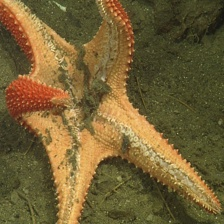
\includegraphics[width=1.7cm]{img/animal1}};
    \node[layer, minimum height=1.45cm] (l1) at (1.55,0) {};
    \node[layer, minimum height=1.05cm, fill=marineblue!30] (l2) at (2.55,0) {};
    \node[layer, minimum height=0.65cm, fill=marineblue!50] (l3) at (3.55,0) {};
    \node[draw=accentorange, fill=accentorange!12, rounded corners=3pt, align=center,
          font=\scriptsize\bfseries, text=accentorange] (out) at (5.0,0) {sea star\\[-1pt]\textit{Hippasteria}};
    \draw[arr] (img) -- (l1); \draw[arr] (l1) -- (l2);
    \draw[arr] (l2) -- (l3);  \draw[arr] (l3) -- (out);
    \foreach \x/\t in {0/ROV image, 1.55/edges, 2.55/{spines,\\[-2pt]textures}, 3.55/{arms,\\[-2pt]body plan}}
      \node[anchor=north, align=center, darkgray, text width=1.1cm] at (\x,-0.9) {\t};
  \end{tikzpicture}\\[6pt]
  \raggedright\small
  \begin{itemize}
    \item \textbf{Too much footage, too few experts.} Underwater robots film for
          hours on every dive -- labelling it by hand is the bottleneck.
    \item \textbf{A CNN learns its own characters} -- edges $\to$ textures $\to$ body
          parts -- from labelled examples, much like a student learning an
          identification key.
    \item \textbf{It does not replace you:} the CNN pre-sorts, the biologist checks.
  \end{itemize}
\end{column}
\begin{column}{0.40\linewidth}
  \begin{infobox}{It already works in this project}
    \small
    A ready-made CNN + a simple classifier, 79 deep-sea taxa:\\[4pt]
    \begin{tabular}{@{}lr@{}}
      guessing the commonest label & \textbf{1\,\%}\\
      raw pixels                   & \textbf{46\,\%}\\
      CNN features                 & \textbf{\textcolor{accentgreen}{65\,\%}}\\
    \end{tabular}\\[4pt]
    {\scriptsize\color{darkgray} our reference run, random test split}
  \end{infobox}
  \vspace{4pt}
  \begin{ideabox}{Your turn}
    \small Which characters do \emph{you} use to tell two species apart --
    and could a camera even see them?
  \end{ideabox}
\end{column}
\end{columns}
\end{frame}

%% ---- Slide 2: The FathomNet 2025 challenge ----
\begin{frame}{The FathomNet 2025 Challenge}
\begin{columns}[T]
\begin{column}{0.47\linewidth}
  \centering
  \setlength{\tabcolsep}{1pt}\renewcommand{\arraystretch}{0}
  \begin{tabular}{cccc}
    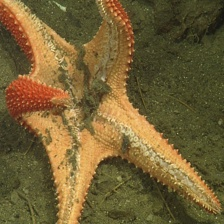
\includegraphics[width=1.55cm,height=1.55cm]{img/animal1} &
    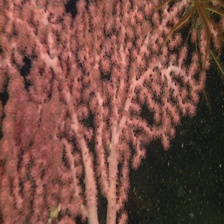
\includegraphics[width=1.55cm,height=1.55cm]{img/animal2} &
    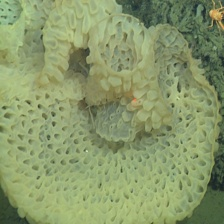
\includegraphics[width=1.55cm,height=1.55cm]{img/animal3} &
    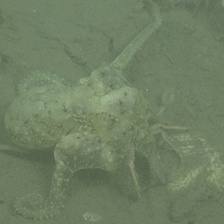
\includegraphics[width=1.55cm,height=1.55cm]{img/animal4} \\[1pt]
    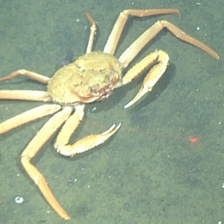
\includegraphics[width=1.55cm,height=1.55cm]{img/animal5} &
    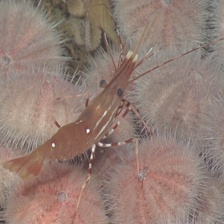
\includegraphics[width=1.55cm,height=1.55cm]{img/animal6} &
    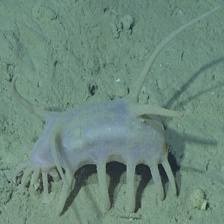
\includegraphics[width=1.55cm,height=1.55cm]{img/animal7} &
    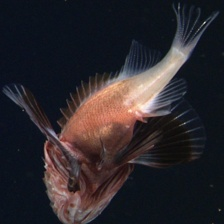
\includegraphics[width=1.55cm,height=1.55cm]{img/animal8} \\
  \end{tabular}\\[5pt]
  {\tiny\color{darkgray} sea star · bubblegum coral · glass sponge · octopus ·
   crab · prawn · sea pig · rockfish \quad (images: FathomNet / MBARI)}\\[6pt]
  \raggedright\small
  \textbf{\color{marineblue}23{,}664} expert-labelled animals \;·\;
  \textbf{\color{marineblue}79} taxa \;·\; \textbf{\color{marineblue}7} phyla \;·\;
  \textbf{\color{marineblue}1{,}465} ROV dives
\end{column}
\begin{column}{0.49\linewidth}
  \small
  \textbf{The task:} name the animal in each box -- as deep in the tree of life as you can.\\[4pt]
  \textbf{The score is biological:} mixing up two sea stars is a small mistake,
  sea star vs.\ coral a big one.\\[4pt]
  \textbf{The catch:} the winning models reach $\approx$\,98\,\% on their training images,
  but only \textcolor{accentred}{\textbf{57--61\,\%}} on dives they have never seen.\\[6pt]
  \begin{ideabox}{Your ideas wanted}
    \small
    \begin{itemize}
      \item Which animals would \emph{you} find hard -- and why?
      \item Which mistakes are acceptable for your research?
      \item What else would help -- depth, location, behaviour, \dots?
      \item What would \emph{you} like to ask this data?
    \end{itemize}
  \end{ideabox}
\end{column}
\end{columns}
\end{frame}

%% (needs the colours and the infobox/ideabox from fathomnet_motivation.tex).
%% =====================================================================

%% ---- Slide 1: Why CNNs? ----
\begin{frame}{Why CNNs? \,--\, Teaching a computer to look like a biologist}
\begin{columns}[T]
\begin{column}{0.56\linewidth}
  \centering
  \begin{tikzpicture}[
      every node/.style={font=\scriptsize},
      layer/.style={draw=marineblue, fill=marineblue!15, minimum width=0.42cm},
      arr/.style={-{Stealth[scale=0.8]}, thick, marineblue}]
    \node[inner sep=0, draw=marineblue, line width=0.8pt] (img) at (0,0)
      {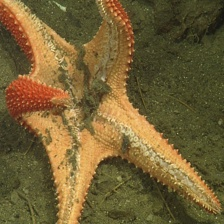
\includegraphics[width=1.7cm]{img/animal1}};
    \node[layer, minimum height=1.45cm] (l1) at (1.55,0) {};
    \node[layer, minimum height=1.05cm, fill=marineblue!30] (l2) at (2.55,0) {};
    \node[layer, minimum height=0.65cm, fill=marineblue!50] (l3) at (3.55,0) {};
    \node[draw=accentorange, fill=accentorange!12, rounded corners=3pt, align=center,
          font=\scriptsize\bfseries, text=accentorange] (out) at (5.0,0) {sea star\\[-1pt]\textit{Hippasteria}};
    \draw[arr] (img) -- (l1); \draw[arr] (l1) -- (l2);
    \draw[arr] (l2) -- (l3);  \draw[arr] (l3) -- (out);
    \foreach \x/\t in {0/ROV image, 1.55/edges, 2.55/{spines,\\[-2pt]textures}, 3.55/{arms,\\[-2pt]body plan}}
      \node[anchor=north, align=center, darkgray, text width=1.1cm] at (\x,-0.9) {\t};
  \end{tikzpicture}\\[6pt]
  \raggedright\small
  \begin{itemize}
    \item \textbf{Too much footage, too few experts.} Underwater robots film for
          hours on every dive -- labelling it by hand is the bottleneck.
    \item \textbf{A CNN learns its own characters} -- edges $\to$ textures $\to$ body
          parts -- from labelled examples, much like a student learning an
          identification key.
    \item \textbf{It does not replace you:} the CNN pre-sorts, the biologist checks.
  \end{itemize}
\end{column}
\begin{column}{0.40\linewidth}
  \begin{infobox}{It already works in this project}
    \small
    A ready-made CNN + a simple classifier, 79 deep-sea taxa:\\[4pt]
    \begin{tabular}{@{}lr@{}}
      guessing the commonest label & \textbf{1\,\%}\\
      raw pixels                   & \textbf{46\,\%}\\
      CNN features                 & \textbf{\textcolor{accentgreen}{65\,\%}}\\
    \end{tabular}\\[4pt]
    {\scriptsize\color{darkgray} our reference run, random test split}
  \end{infobox}
  \vspace{4pt}
  \begin{ideabox}{Your turn}
    \small Which characters do \emph{you} use to tell two species apart --
    and could a camera even see them?
  \end{ideabox}
\end{column}
\end{columns}
\end{frame}

%% ---- Slide 2: The FathomNet 2025 challenge ----
\begin{frame}{The FathomNet 2025 Challenge}
\begin{columns}[T]
\begin{column}{0.47\linewidth}
  \centering
  \setlength{\tabcolsep}{1pt}\renewcommand{\arraystretch}{0}
  \begin{tabular}{cccc}
    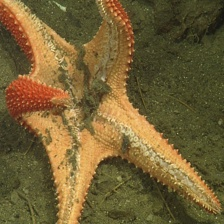
\includegraphics[width=1.55cm,height=1.55cm]{img/animal1} &
    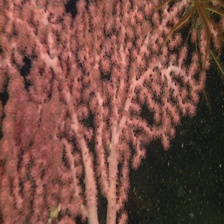
\includegraphics[width=1.55cm,height=1.55cm]{img/animal2} &
    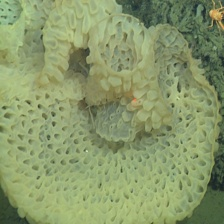
\includegraphics[width=1.55cm,height=1.55cm]{img/animal3} &
    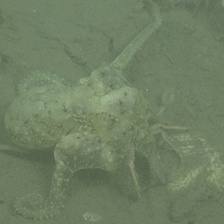
\includegraphics[width=1.55cm,height=1.55cm]{img/animal4} \\[1pt]
    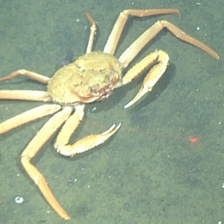
\includegraphics[width=1.55cm,height=1.55cm]{img/animal5} &
    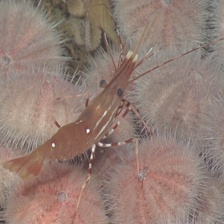
\includegraphics[width=1.55cm,height=1.55cm]{img/animal6} &
    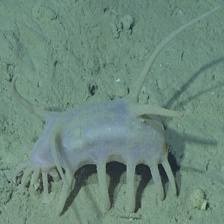
\includegraphics[width=1.55cm,height=1.55cm]{img/animal7} &
    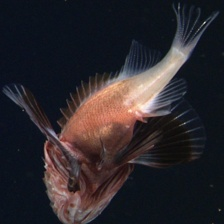
\includegraphics[width=1.55cm,height=1.55cm]{img/animal8} \\
  \end{tabular}\\[5pt]
  {\tiny\color{darkgray} sea star · bubblegum coral · glass sponge · octopus ·
   crab · prawn · sea pig · rockfish \quad (images: FathomNet / MBARI)}\\[6pt]
  \raggedright\small
  \textbf{\color{marineblue}23{,}664} expert-labelled animals \;·\;
  \textbf{\color{marineblue}79} taxa \;·\; \textbf{\color{marineblue}7} phyla \;·\;
  \textbf{\color{marineblue}1{,}465} ROV dives
\end{column}
\begin{column}{0.49\linewidth}
  \small
  \textbf{The task:} name the animal in each box -- as deep in the tree of life as you can.\\[4pt]
  \textbf{The score is biological:} mixing up two sea stars is a small mistake,
  sea star vs.\ coral a big one.\\[4pt]
  \textbf{The catch:} the winning models reach $\approx$\,98\,\% on their training images,
  but only \textcolor{accentred}{\textbf{57--61\,\%}} on dives they have never seen.\\[6pt]
  \begin{ideabox}{Your ideas wanted}
    \small
    \begin{itemize}
      \item Which animals would \emph{you} find hard -- and why?
      \item Which mistakes are acceptable for your research?
      \item What else would help -- depth, location, behaviour, \dots?
      \item What would \emph{you} like to ask this data?
    \end{itemize}
  \end{ideabox}
\end{column}
\end{columns}
\end{frame}

\end{document}
